% Day 6 notes, SC Quantathon v3 Bootcamp. Build: latexmk -pdf notes.tex
\documentclass[11pt]{article}

\usepackage[margin=1in]{geometry}
\usepackage{lmodern}
\usepackage[T1]{fontenc}
\usepackage{microtype}
\usepackage{amsmath,amssymb}
\usepackage{braket}
\usepackage{graphicx}
\usepackage{booktabs}
\usepackage{caption}
\usepackage{listings}
\usepackage{xcolor}
\usepackage[hidelinks]{hyperref}

\captionsetup{font=small,labelfont=bf}
\graphicspath{{figures/}}

\lstset{
  language=Python,
  basicstyle=\ttfamily\small,
  keywordstyle=\color{blue!60!black},
  commentstyle=\color{gray},
  stringstyle=\color{green!40!black},
  showstringspaces=false,
  frame=single,
  framerule=0.3pt,
  rulecolor=\color{gray!50},
  xleftmargin=1em,
  aboveskip=0.6em,
  belowskip=0.6em,
}

\newcommand{\code}[1]{\texttt{#1}}

\title{Day 6: Variational Algorithms: VQE and QAOA}
\author{SC Quantathon v3 Bootcamp \\ Clemson Quantum Club}
\date{}

\begin{document}
\maketitle

\noindent
The algorithms that run on today's noisy processors share one shape: a short parameterized circuit, an expectation value read off it, and a classical optimizer that adjusts the parameters. These notes build that loop for a molecule's ground-state energy, then ask the three questions that decide whether it works in practice: how the optimizer should move, what noise does to the energy, and how the circuit should be chosen. They end with the same loop on a graph problem. They follow the order of the Day~6 notebook.

\section{Parameterized circuits and the ansatz}

A rotation gate takes an angle. Leave the angle as a symbol and the circuit becomes a function of it. Qiskit's \code{Parameter} makes one symbol, \code{ParameterVector} makes many, and \code{assign\_parameters} binds numbers to them. A parameterized circuit used as the family of states an algorithm searches through is called an \emph{ansatz}, and the state it prepares is written $\ket{\psi(\vec\theta)}$.

The notebook's ansatz is the \emph{hardware-efficient} one of Figure~\ref{fig:ansatz}: a layer of $R_y(\theta_k)$ on every qubit, a ladder of CNOTs, and a final rotation layer, repeated \code{reps} times. With $n$ qubits and \code{reps} entangling layers it has $n(\text{reps}+1)$ parameters, four for the two-qubit, one-layer version used below. It is called hardware efficient because every gate in it is cheap on a real chip; nothing about it is tailored to the problem, which is both its convenience and its weakness (Section~\ref{sec:ansatz}).

\begin{figure}[h]
\centering
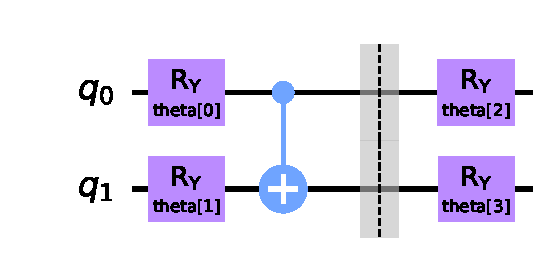
\includegraphics[width=0.5\textwidth]{ansatz}
\caption{The hardware-efficient ansatz for two qubits and one entangling layer: $R_y$ on each qubit, a CNOT, $R_y$ on each qubit, four parameters in all.}
\label{fig:ansatz}
\end{figure}

\section{Hamiltonians and the variational principle}

A physical system's energy is an observable, its \emph{Hamiltonian} $H$, and on qubits it is written as a sum of Pauli strings with real coefficients, exactly the \code{SparsePauliOp} objects of Day~4. Its eigenvalues are the allowed energies and the smallest, $E_0$, is the \emph{ground-state energy}. Expanding any state in the eigenbasis, $\ket{\psi} = \sum_k c_k\ket{E_k}$, gives
\begin{equation}
\braket{\psi|H|\psi} = \sum_k |c_k|^2 E_k \;\ge\; E_0 \sum_k |c_k|^2 = E_0 ,
\label{eq:variational}
\end{equation}
with equality only when all the weight sits in the ground eigenspace. This is the \emph{variational principle}: every state's energy is an upper bound on $E_0$, so minimizing the energy over an ansatz can only approach $E_0$ from above, and whatever minimum is reached is a rigorous upper bound on the true value.

The principle has a second consequence that explains why VQE energies converge so much faster than the states behind them. Write a nearly correct state as $\ket{\psi} = (\ket{E_0} + \varepsilon\ket{\varphi})/\sqrt{1+\varepsilon^2}$ with $\ket{\varphi}$ orthogonal to the ground state. Then
\begin{equation}
\braket{\psi|H|\psi} - E_0 = \frac{\varepsilon^2}{1+\varepsilon^2}\big(\braket{\varphi|H|\varphi} - E_0\big),
\label{eq:quadratic}
\end{equation}
with no term linear in $\varepsilon$, because the cross terms $\braket{E_0|H|\varphi}$ vanish. A state that is wrong by ten percent has an energy wrong by about one percent of the gap. The error in the energy is second order in the error of the state, which is what makes a rough ansatz useful.

The notebook's Hamiltonian is the hydrogen molecule $\mathrm{H}_2$ at its equilibrium bond length of 0.735~\AA, reduced to two qubits by symmetry. The coefficients are the standard values generated by Qiskit Nature (STO-3G basis, parity mapping) and used throughout Qiskit's tutorials:
\begin{equation}
H_{\rm mol} = -1.0524\,II + 0.3979\,IZ - 0.3979\,ZI - 0.0113\,ZZ + 0.1809\,XX .
\label{eq:h2}
\end{equation}
Its $4\times4$ matrix has eigenvalues $-1.8573$, $-1.2446$, $-0.8827$, and $-0.2249$ hartree, so $E_0 = -1.857275$ hartree. This is the electronic energy; adding the nuclear repulsion of the two protons at this distance, $+0.7199$ hartree, gives the molecular ground-state energy $-1.1374$ hartree, the number chemistry tables quote. For two qubits \code{np.linalg.eigvalsh} gives this in a microsecond; the point of the quantum algorithm is that the matrix has $2^n$ rows and the shortcut ends around 30 qubits (Day~4).

\section{VQE}

The \emph{variational quantum eigensolver} (VQE) minimizes
\begin{equation}
E(\vec\theta) = \braket{\psi(\vec\theta)|H|\psi(\vec\theta)}
\label{eq:vqe}
\end{equation}
over the ansatz parameters. The quantum processor, or here the Estimator, evaluates Eq.~\eqref{eq:vqe} for a given $\vec\theta$; a classical optimizer chooses the next $\vec\theta$; and by Eq.~\eqref{eq:variational} the running minimum is always an upper bound on $E_0$.

\subsection{One parameter}

With one parameter the whole landscape can be drawn. The ansatz $X$ on qubit~0, then $R_y(\theta)$ on qubit~1, then CNOT from qubit~1 to qubit~0 sweeps through the states $\cos\frac\theta2\ket{01} + \sin\frac\theta2\ket{10}$ up to sign, and this one-parameter family happens to contain the $\mathrm{H}_2$ ground state (Section~\ref{sec:ansatz} says why). Figure~\ref{fig:landscape} is $E(\theta)$ over a full turn: a single smooth well whose bottom, at $\theta = -0.209$ on the grid, sits at $-1.85719$ hartree, within $10^{-4}$ of $E_0$. The exact ground state, from \code{eigh}, is $0.9938\ket{01} - 0.1115\ket{10}$, so the true minimum sits at $\theta = 2\arctan(-0.1115/0.9938) = -0.223$, one grid step from the sampled point; the $10^{-4}$ is the curvature of the well over that step, Eq.~\eqref{eq:quadratic} at work. The Hartree-Fock state $\ket{01}$ alone carries 99\% of the weight, and the 1\% of $\ket{10}$ is the electron correlation that lowers the energy from $-1.8370$ to $-1.8573$ hartree.

\begin{figure}[h]
\centering
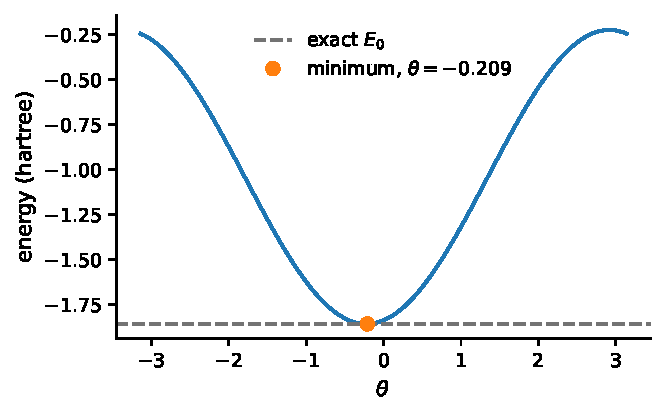
\includegraphics[width=0.58\textwidth]{landscape}
\caption{The energy landscape of the one-parameter ansatz for the $\mathrm{H}_2$ Hamiltonian, Eq.~\eqref{eq:h2}. The dashed line is the exact ground-state energy.}
\label{fig:landscape}
\end{figure}

\subsection{Four parameters}

With the four-parameter ansatz of Figure~\ref{fig:ansatz} the landscape cannot be drawn, and an optimizer walks it instead. COBYLA is the usual first choice because it needs no gradients. Starting from random angles, Figure~\ref{fig:vqe} shows every energy it requested: 105 evaluations, ending at $-1.857275$ hartree, within $2\times10^{-9}$ of the exact value.

\begin{figure}[h]
\centering
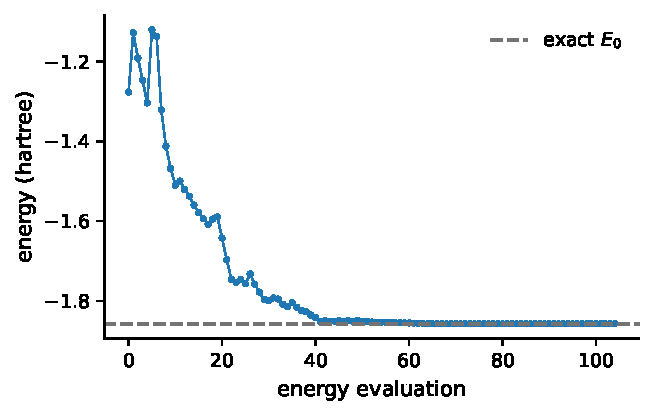
\includegraphics[width=0.58\textwidth]{vqe_convergence}
\caption{VQE on $\mathrm{H}_2$ with the hardware-efficient ansatz and COBYLA: the energy at every evaluation, converging to $E_0$.}
\label{fig:vqe}
\end{figure}

\section{Gradients and optimizers}

\subsection{The parameter-shift rule}

Every gate in the ansatz is $R_y(\theta) = e^{-i\theta Y/2} = \cos\frac\theta2\,I - i\sin\frac\theta2\,Y$ (Day~4). Hold every angle but $\theta_k$ fixed. The state is then linear in $\cos\frac{\theta_k}2$ and $\sin\frac{\theta_k}2$, so the energy, a quadratic form in the state, is a combination of $\cos^2\frac{\theta_k}2$, $\sin^2\frac{\theta_k}2$, and $\sin\frac{\theta_k}2\cos\frac{\theta_k}2$, which the half-angle identities turn into
\begin{equation}
E(\theta_k) = a + b\cos\theta_k + c\sin\theta_k
\label{eq:sinusoid}
\end{equation}
for some constants $a, b, c$ that depend on the other angles. Its derivative is $-b\sin\theta_k + c\cos\theta_k$. Evaluating Eq.~\eqref{eq:sinusoid} a quarter turn to either side gives $E(\theta_k \pm \frac\pi2) = a \mp b\sin\theta_k \pm c\cos\theta_k$, and half their difference is the derivative:
\begin{equation}
\frac{\partial E}{\partial\theta_k} = \frac12\Big[E\big(\theta_k + \tfrac\pi2\big) - E\big(\theta_k - \tfrac\pi2\big)\Big] .
\label{eq:shift}
\end{equation}
This is the \emph{parameter-shift rule}. It is exact, not an approximation; the notebook checks it against a central finite difference with step $10^{-4}$ and the two agree to $4\times10^{-10}$. On hardware the difference matters: a finite difference divides the shot noise of two nearby energies by a small step, while Eq.~\eqref{eq:shift} divides the noise of two well-separated energies by 2. A full gradient of $m$ parameters costs $2m$ energy evaluations.

\subsection{Three optimizers on the same problem}

\emph{Gradient descent} steps against the gradient, $\vec\theta \leftarrow \vec\theta - \eta\,\nabla E$, at $2m + 1$ evaluations per step (the gradient plus the new energy). \emph{SPSA}, simultaneous perturbation stochastic approximation, replaces the gradient by a two-point estimate along a random direction $\vec\Delta$ whose entries are $\pm1$:
\begin{equation}
\hat g_k = \frac{E(\vec\theta + c_k\vec\Delta) - E(\vec\theta - c_k\vec\Delta)}{2c_k}\,\vec\Delta ,\qquad
\vec\theta \leftarrow \vec\theta - a_k\,\hat g_k ,\qquad
a_k = \frac{a}{(k + 1 + A)^{0.602}},\quad c_k = \frac{c}{(k+1)^{0.101}} .
\label{eq:spsa}
\end{equation}
Two evaluations per step no matter how many parameters (the notebook's third call per step only records the energy for the plot), an estimate that is wrong in direction on any one step but unbiased on average, and gains that shrink at Spall's recommended rates. The unbiasedness is a one-line calculation: expanding $E(\vec\theta \pm c\vec\Delta)$ to first order gives $\hat g_k \approx \vec\Delta\,(\vec\Delta\cdot\nabla E) = \sum_j \Delta_k\Delta_j\,\partial_jE$, and since the entries of $\vec\Delta$ are independent $\pm1$, the average of $\Delta_k\Delta_j$ is 1 for $j = k$ and 0 otherwise, leaving $\partial_kE$. \emph{COBYLA} (constrained optimization by linear approximation) keeps a simplex of $m + 1$ recent points, fits a linear model of the energy through them, steps to the minimum of that model inside a trust region, and shrinks the region when the step disappoints; it never touches a gradient, which is why it needs only about one evaluation per step. All three start from the same random point; Table~\ref{tab:opt} and Figure~\ref{fig:opt} show the runs.

\begin{table}[h]
\centering
\small
\begin{tabular}{@{}lllll@{}}
\toprule
optimizer & settings & steps & energy evaluations & final error (hartree) \\
\midrule
gradient descent & $\eta = 1$, parameter-shift gradient & 100 & 901 & $< 10^{-12}$ \\
SPSA & $a = 2$, $c = 0.2$, $A = 10$ & 200 & 601 & $3\times10^{-6}$ \\
COBYLA & \code{maxiter = 200} & 105 & 105 & $6\times10^{-9}$ \\
\bottomrule
\end{tabular}
\caption{Three optimizers on the four-parameter $\mathrm{H}_2$ problem from the same starting angles.}
\label{tab:opt}
\end{table}

\begin{figure}[h]
\centering
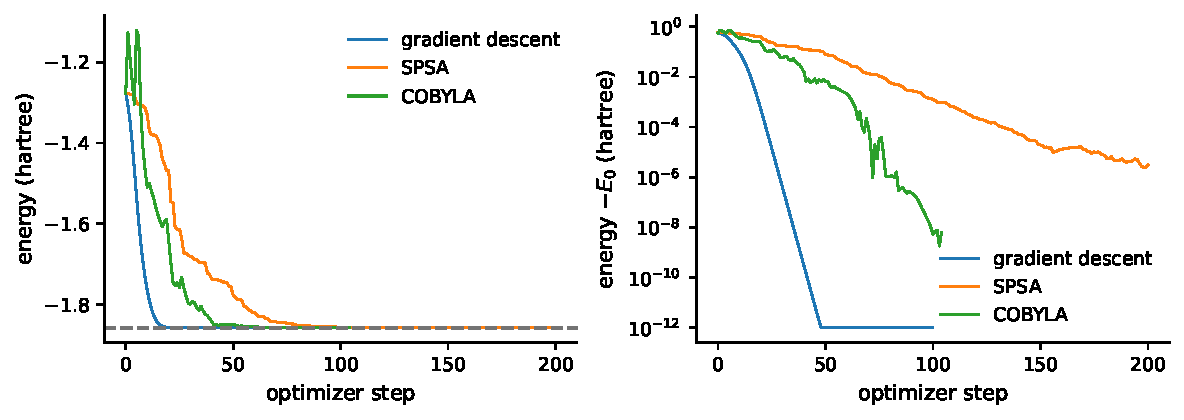
\includegraphics[width=0.98\textwidth]{optimizers}
\caption{Energy per optimizer step (left) and distance from $E_0$ on a log scale (right) for gradient descent, SPSA, and COBYLA.}
\label{fig:opt}
\end{figure}

Gradient descent is the most predictable and the most expensive per step. SPSA takes many small, noisy steps at two evaluations each and still lands within microhartrees. COBYLA is the cheapest here, on an exact energy; with shot noise its linear models are fooled more easily, which is why SPSA and the parameter-shift rule are the standard tools once the energy comes from a device.

\section{VQE under noise}

\subsection{An energy from counts}

The Estimator read $\braket{H}$ off the state vector. A processor has to assemble it from counts, one measurement basis per group of commuting terms. In Eq.~\eqref{eq:h2}, $IZ$, $ZI$, and $ZZ$ are diagonal in the computational basis, so one circuit measured in the $Z$ basis serves all three:
\begin{equation}
\braket{Z_0} = P(q_0 = 0) - P(q_0 = 1),\qquad \braket{Z_1} = P(q_1 = 0) - P(q_1 = 1),\qquad \braket{Z_0Z_1} = P(\text{agree}) - P(\text{differ}),
\label{eq:zterms}
\end{equation}
and $XX$ needs a Hadamard on each qubit before measuring (Day~4), after which the same agree-minus-differ rule gives $\braket{X_0X_1}$. The energy is $E = \sum_P c_P\braket{P}$ with the coefficients of Eq.~\eqref{eq:h2}. Grouping terms that share a basis is the general strategy: the four terms of $H_{\rm mol}$ need two measurement circuits, and a molecular Hamiltonian with thousands of Pauli terms is partitioned into sets of mutually commuting strings, one circuit per set. Each $\braket{P}$ estimated from $N$ shots carries a standard error of $\sqrt{(1 - \braket{P}^2)/N}$ (Day~4), and the coefficients weight those errors into the energy,
\begin{equation}
\sigma_E^2 \approx \sum_P c_P^2\,\frac{1 - \braket{P}^2}{N} .
\label{eq:shotnoise}
\end{equation}
In the ground state $\braket{IZ} = -0.975$, $\braket{ZI} = 0.975$, $\braket{ZZ} = -1.000$, and $\braket{XX} = -0.222$, so at $N = 1000$ per basis Eq.~\eqref{eq:shotnoise} gives $\sigma_E = 0.0068$ hartree; the $ZZ$ term contributes nothing because every shot returns the same value, $Z_0Z_1 = -1$, and the $XX$ term, far from an eigenvalue, contributes most. Eq.~\eqref{eq:shotnoise} treats the terms as independent, and here they are not: $IZ$, $ZI$, and $ZZ$ come from the same shots, and in this state the estimates of $\braket{Z_0}$ and $\braket{Z_1}$ move in opposite directions while their coefficients have opposite signs, so their errors add. Resampling the notebook's estimator 20\,000 times gives the true figure, $\sigma_E = 0.0078$ hartree. The notebook's estimate came out $0.0042$ hartree below the exact value, well within one $\sigma_E$, and below, because a shot estimate is a statistic, not the energy of a state, so Eq.~\eqref{eq:variational} does not bound it. Chemical accuracy, $0.0016$ hartree, would need about 24 times more shots.

\subsection{Gate error, readout error, and mitigation}

Day~5's noisy simulator of \code{ibm\_sherbrooke} adds relaxation during every gate, depolarizing error at the calibrated rates, and readout error. A level-3 transpilation places the two logical qubits on physical qubits 123 and 124, where the ISA circuit has depth 13 with one \code{ecr}; every circuit in this section is then pinned to those qubits so that one readout calibration applies to all of them. The noisy runs use 10\,000 shots, enough to put statistical noise well below the hardware bias. The confusion matrix measured on the pair has diagonal entries 0.989, 0.988, 0.988, 0.986, and Day~5's inversion, applied to each of the two measured distributions before Eq.~\eqref{eq:zterms}, gives the mitigated energy. Table~\ref{tab:noise} and Figure~\ref{fig:noise} collect the four numbers.

\begin{table}[h]
\centering
\small
\begin{tabular}{@{}lll@{}}
\toprule
energy at the optimal angles & hartree & error \\
\midrule
exact (state vector) & $-1.8573$ & \\
1000 shots per basis, no other noise & $-1.8615$ & $-0.0042$ \\
noisy simulator, 10\,000 shots & $-1.8463$ & $+0.0110$ \\
noisy simulator, readout mitigated & $-1.8567$ & $+0.0006$ \\
\bottomrule
\end{tabular}
\caption{The same energy four ways. The noisy energy lies above $E_0$ because noise mixes higher-energy states into the prepared one.}
\label{tab:noise}
\end{table}

\begin{figure}[h]
\centering
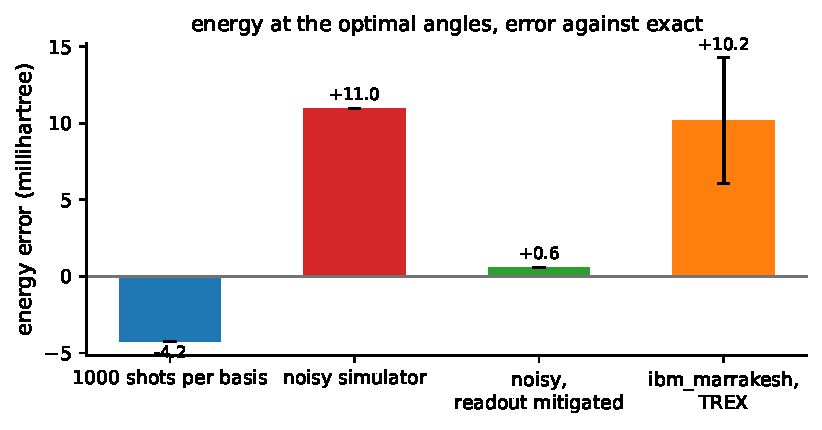
\includegraphics[width=0.6\textwidth]{noisy_vqe}
\caption{Error of the estimated energies against the exact value, in millihartree: the three rows of Table~\ref{tab:noise} and the live run of Section~\ref{sec:live}, with its statistical error bar.}
\label{fig:noise}
\end{figure}

The noisy energy lies above the exact one, unlike the shot estimate, and that is what gate noise does: a noisy circuit prepares a mixture of states, whose energy is a weighted average $\sum_k p_k E_k$ of the energies of its components, and every one of those is at least $E_0$ by Eq.~\eqref{eq:variational}. Gate and relaxation noise therefore look like an ansatz that is not quite good enough, and mitigation moves the number back down toward the bound. Readout error and the remaining shot noise are not bound this way, since they act on the counts rather than on the state, which is why the mitigated number can in principle land on either side. Readout mitigation removes most of the 11 millihartree of error. The residual, $0.6$ millihartree, is smaller than the shot noise of a 10\,000-shot estimate, about $2.5$ millihartree by Eq.~\eqref{eq:shotnoise}, so it is consistent with zero: whatever the \code{ecr} gate and the relaxation during it contribute on the snapshot is below what this run can resolve, and Day~5's zero-noise extrapolation is the tool for it when it is not. Chemical accuracy, the precision needed to predict reaction rates, is 1.6 millihartree; the mitigated number lands inside it here, within its error bar. The runtime Estimator performs the readout calibration itself when \code{resilience\_level = 1} is set; in local testing mode that option is ignored, which is why the notebook does it by hand.

\subsection{The energy on the live machine}
\label{sec:live}

The notebook's last section sends the same circuit, at the optimal angles, to the least busy live processor through the runtime Estimator with \code{resilience\_level = 1}, which applies the readout calibration of Section~5.2 automatically. The recorded run went to \code{ibm\_marrakesh}, physical qubits 14 and 15, an ISA circuit of depth 11 with one \code{cz}, at the Estimator's default of 4096 shots, and returned
\begin{equation}
E_{\rm marrakesh} = -1.8471 \pm 0.0041\ \text{hartree},\qquad E_{\rm marrakesh} - E_0 = +0.0102\ \text{hartree},
\label{eq:live}
\end{equation}
the error bar being the shot noise the runtime reports. Against the exact $-1.8573$ and the snapshot's readout-mitigated $-1.8567$, the device sits ten millihartree high, two and a half error bars above the exact value and about six times chemical accuracy (Figure~\ref{fig:noise}). With readout already corrected by TREX, what remains is, by elimination, the \code{cz} gate and relaxation during the circuit, the part Day~5 attacked with zero-noise extrapolation. Switching that on in the runtime options (\code{resilience.zne\_mitigation = True}) is the natural next step, at the price of several times the QPU time.

\section{Ansatz design and the dissociation curve}
\label{sec:ansatz}

\subsection{Two ansätze for the same molecule}

The four-parameter ansatz found the ground state, but so did the one-parameter circuit of Section~3.1, and it is not luck. $H_{\rm mol}$ in Eq.~\eqref{eq:h2} couples $\ket{01}$ only to $\ket{10}$, through the $XX$ term, and $\ket{00}$ only to $\ket{11}$; the ground state lives in the first pair. The one-parameter circuit is the two-qubit form of the \emph{unitary coupled cluster} ansatz that O'Malley et al.\ ran on hardware,
\begin{equation}
e^{-i\theta X_0Y_1}\ket{01} = \cos\theta\,\ket{01} + \sin\theta\,\ket{10},
\label{eq:ucc}
\end{equation}
since $X_0Y_1\ket{01} = i\ket{10}$ and $(X_0Y_1)^2 = I$. It starts at the Hartree-Fock state $\ket{01}$ when $\theta = 0$, reaches every state in the pair, and never leaves it. A \emph{problem-inspired} ansatz like this has nothing to learn that the physics already rules out. A \emph{hardware-efficient} ansatz is generic: it covers states the problem never needs, and its gradients shrink with qubit count (Day~7 measures that). From the same starting point, COBYLA needs 105 evaluations to reach $E_0$ with the four-parameter ansatz (error $2\times10^{-9}$) and 23 with the one-parameter ansatz (error $2\times10^{-10}$).

\subsection{The dissociation curve of \texorpdfstring{$\mathrm{H}_2$}{H2}}

A single energy is not what chemistry wants; the energy as a function of bond length $R$ is. O'Malley et al.\ (2016) tabulated the two-qubit Hamiltonian at 54 bond lengths,
\begin{equation}
H(R) = g_0\,I + g_1\,Z_0 + g_2\,Z_1 + g_3\,Z_0Z_1 + g_4\,X_0X_1 + g_4\,Y_0Y_1 ,
\label{eq:hr}
\end{equation}
in the STO-6G basis with the Bravyi-Kitaev mapping and with the nuclear repulsion already inside $g_0$. The $Y_0Y_1$ coefficient equals the $X_0X_1$ one at every $R$, and $(X_0X_1 + Y_0Y_1)$ couples $\ket{01}$ to $\ket{10}$ with matrix element $2g_4$ while annihilating $\ket{00}$ and $\ket{11}$, so Eq.~\eqref{eq:ucc} again contains the ground state at every $R$. Because the basis differs from the STO-3G one behind Eq.~\eqref{eq:h2}, the equilibrium energies differ too, $-1.1456$ against $-1.1373$ hartree: the number depends on the basis set, and only the shape of the curve is comparable between them.

The notebook runs the one-parameter VQE at 45 bond lengths from 0.30 to 2.50~\AA\ (Figure~\ref{fig:dissociation}). It matches the exact eigenvalue of Eq.~\eqref{eq:hr} to $4\times10^{-13}$ hartree everywhere, and the minimum falls at $R = 0.75$~\AA\ with energy $-1.1456$ hartree. The Hartree-Fock state alone misses by $0.021$ hartree at equilibrium and by $0.233$ hartree at 2.5~\AA, where one configuration cannot describe two separating atoms; the single angle captures that correlation at every $R$. The failure has a simple cause. In the molecular-orbital picture the Hartree-Fock state puts both electrons in the bonding orbital, which spreads each electron equally over both atoms, so at any separation it assigns half its weight to configurations with both electrons on the same atom. Near equilibrium that is a fair description of a covalent bond; at large $R$ it describes a pair of ions, which costs a large energy. The second configuration, $\ket{10}$, is the one that cancels the ionic part, and its weight in the ground state grows from about 1\% at equilibrium to 40\% at 2.5~\AA, heading toward one half as the atoms separate completely. That growth is exactly what the angle $\theta$ tracks. The depth of the well, $E(2.5\,\text{\AA}) - E_{\min} = 0.2007$ hartree or 5.46~eV, overshoots the experimental dissociation energy of 4.75~eV, an error of the minimal basis and not of the algorithm.

\begin{figure}[h]
\centering
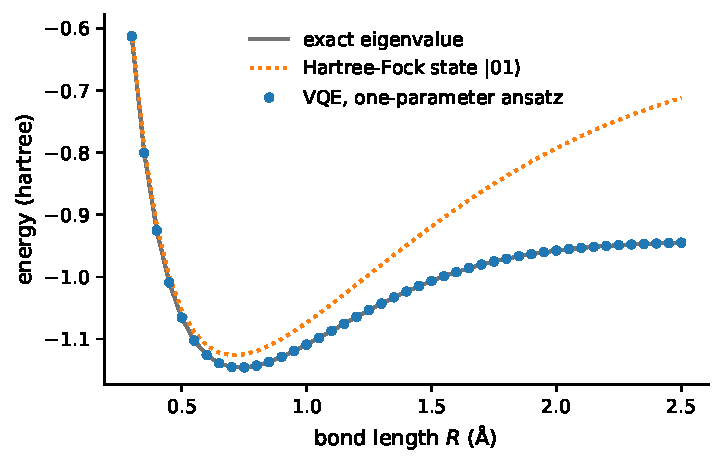
\includegraphics[width=0.62\textwidth]{dissociation}
\caption{$\mathrm{H}_2$ energy against bond length from the O'Malley coefficients: exact eigenvalue, the Hartree-Fock state $\ket{01}$, and VQE with the one-parameter ansatz at 45 bond lengths.}
\label{fig:dissociation}
\end{figure}

\section{QAOA}

\subsection{MaxCut as a Hamiltonian}

Take a graph and color every node 0 or 1. An edge is \emph{cut} when its two ends have different colors, and \emph{MaxCut} asks for the coloring that cuts the most edges. It is easy to check a coloring and NP-hard to find the best one in general. Encode a coloring as a bitstring, one qubit per node. Since $Z_iZ_j$ is $+1$ when bits $i$ and $j$ agree and $-1$ when they differ, the number of cut edges is the observable
\begin{equation}
C = \sum_{(i,j)\in E} \frac{1 - Z_iZ_j}{2} ,
\label{eq:maxcut}
\end{equation}
diagonal in the computational basis with the cut value of each coloring as its eigenvalue. The best coloring is the eigenvector with the largest eigenvalue. The same substitution, $x_i = (1 - Z_i)/2$, turns any \emph{QUBO} (quadratic unconstrained binary optimization, $\min x^{\mathsf T}Qx$ over bits) into a Hamiltonian, which is why optimization problems are a natural target for these methods. A two-bit example shows the mechanics. The cost $x_0 + x_1 - 3x_0x_1$, which is $0, 1, 1, -1$ on the inputs $00, 10, 01, 11$, becomes
\begin{equation}
x_0 + x_1 - 3x_0x_1 = \tfrac14\,I + \tfrac14\,(Z_0 + Z_1) - \tfrac34\,Z_0Z_1 ,
\label{eq:qubo}
\end{equation}
and substituting $Z_i = \pm1$ for $x_i = 0, 1$ reproduces the four costs. A linear term in a bit becomes a single $Z$, a product of two bits becomes a $ZZ$, and the constants collect into the identity; the minimum of the QUBO is the smallest eigenvalue of the result, so the same Estimator and optimizer that found a molecule's energy can search for it.

The notebook's graph is a square: four nodes, four edges. Table~\ref{tab:cuts} lists every coloring's cut; the maximum, 4, is reached by the two alternating colorings.

\begin{table}[h]
\centering
\small
\begin{tabular}{@{}ll@{}}
\toprule
cut & colorings \\
\midrule
0 & \code{0000}, \code{1111} \\
2 & \code{0001}, \code{0010}, \code{0100}, \code{1000}, \code{0111}, \code{1011}, \code{1101}, \code{1110}, \code{0011}, \code{0110}, \code{1100}, \code{1001} \\
4 & \code{0101}, \code{1010} \\
\bottomrule
\end{tabular}
\caption{Cut values of all 16 colorings of the square graph.}
\label{tab:cuts}
\end{table}

\subsection{The QAOA circuit}

The \emph{quantum approximate optimization algorithm} (QAOA) uses an ansatz built from the problem. Start in $\ket{+}^{\otimes n}$, the uniform superposition of all colorings. Then alternate two layers $p$ times:
\begin{equation}
\ket{\psi(\vec\gamma,\vec\beta)} = U_B(\beta_p)\,U_C(\gamma_p)\cdots U_B(\beta_1)\,U_C(\gamma_1)\,\ket{+}^{\otimes n}, \qquad U_C(\gamma) = e^{-i\gamma\sum_{(i,j)\in E} Z_iZ_j},\quad U_B(\beta) = e^{-i\beta\sum_i X_i} .
\label{eq:qaoa}
\end{equation}
The \emph{cost layer} $U_C(\gamma)$ is one $R_{zz}(2\gamma)$ gate per edge, since $R_{zz}(\vartheta) = e^{-i\vartheta Z_iZ_j/2}$; up to a global phase it equals $e^{-i\gamma' C}$ with $\gamma' = -2\gamma$, so it gives each coloring a phase proportional to its cut. The \emph{mixer layer} $e^{-i\beta\sum X_i}$ is one $R_x(2\beta)$ per qubit; it moves amplitude between colorings. The $2p$ angles are chosen to maximize $\braket{C}$, which by the same variational logic as Eq.~\eqref{eq:variational} can never exceed the true maximum cut; sampling the optimized state then reads out good colorings.

Unlike the VQE landscape of Section~3, the QAOA landscape in $\vec\gamma, \vec\beta$ has many local optima, so the notebook restarts the optimizer from three random points and keeps the best; on hardware this is standard practice, and good angles found on small instances often transfer to larger ones of the same kind. On the square with $p = 2$, three COBYLA restarts each reached $\braket{C} = 4.000$, the maximum possible. Sampling the optimized state 1000 times gave 483 of \code{0101} and 517 of \code{1010} and nothing else (Figure~\ref{fig:qaoa}): every sample is a perfect cut. On larger graphs the approximation ratio improves with $p$, and each extra layer costs another round of two-qubit gates; whether QAOA can beat the best classical heuristics at useful sizes is an open question.

\begin{figure}[h]
\centering
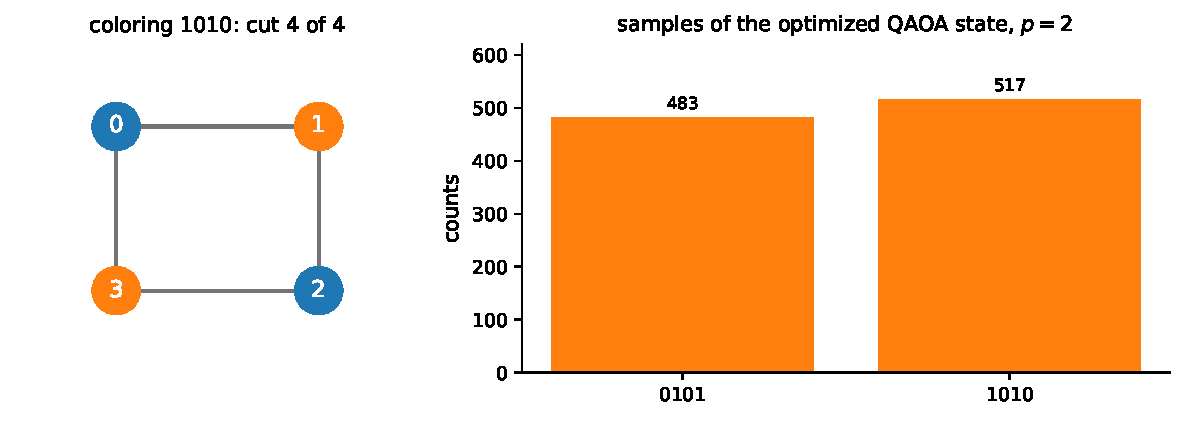
\includegraphics[width=0.95\textwidth]{maxcut_qaoa}
\caption{Left: the square graph colored by the most frequent QAOA sample; every edge is cut. Right: 1000 samples of the optimized $p = 2$ state. Only the two maximum cuts appear.}
\label{fig:qaoa}
\end{figure}

\section{Summary}

\begin{itemize}
\item A parameterized circuit is a circuit with symbolic angles; used as a search space it is an ansatz. The hardware-efficient ansatz has $n(\text{reps}+1)$ parameters.
\item A Hamiltonian is an observable in Pauli strings. The variational principle, Eq.~\eqref{eq:variational}, makes every ansatz energy an upper bound on $E_0$.
\item VQE minimizes the Estimator's energy, Eq.~\eqref{eq:vqe}, with a classical optimizer. On two-qubit $\mathrm{H}_2$, Eq.~\eqref{eq:h2}, COBYLA reaches the electronic energy $E_0 = -1.8573$ hartree in about a hundred evaluations.
\item For rotation gates the energy is a sinusoid in each angle, Eq.~\eqref{eq:sinusoid}, so the parameter-shift rule, Eq.~\eqref{eq:shift}, gives exact gradients from two evaluations per parameter. Gradient descent, SPSA, Eq.~\eqref{eq:spsa}, and COBYLA all reach $E_0$ on the exact energy (Table~\ref{tab:opt}); SPSA's two evaluations per step make it the usual choice under noise.
\item On a processor the energy is assembled from counts in one basis per group of commuting terms, Eq.~\eqref{eq:zterms}. Shot noise, gate error, and readout error each shift it; readout mitigation removed most of the error here (Table~\ref{tab:noise}).
\item On the live machine the runtime's readout mitigation left the VQE energy ten millihartree above exact, Eq.~\eqref{eq:live}, an order of magnitude more than the snapshot's mitigated residual, which that run could not resolve at all.
\item The problem-inspired ansatz, Eq.~\eqref{eq:ucc}, reaches the ground state with one parameter and a fifth of the evaluations. VQE at 45 bond lengths reproduces the $\mathrm{H}_2$ dissociation curve of Eq.~\eqref{eq:hr}, with its minimum at 0.75~\AA\ in the STO-6G basis.
\item MaxCut, and any QUBO, becomes a diagonal Hamiltonian through $Z_iZ_j$ terms, Eq.~\eqref{eq:maxcut}. QAOA alternates cost and mixer layers, Eq.~\eqref{eq:qaoa}, and samples the optimized state; on the square, $p = 2$ finds only perfect cuts.
\end{itemize}

\begin{thebibliography}{9}
\bibitem{peruzzo} A.~Peruzzo et al., ``A variational eigenvalue solver on a photonic quantum processor,'' Nature Communications \textbf{5}, 4213 (2014).
\bibitem{omalley} P.~J.~J. O'Malley et al., ``Scalable quantum simulation of molecular energies,'' Phys. Rev. X \textbf{6}, 031007 (2016). The two-qubit $\mathrm{H}_2$ experiment on hardware and, in its Table~I, the coefficients of Eq.~\eqref{eq:hr}; the coefficients in Eq.~\eqref{eq:h2} are Qiskit Nature's.
\bibitem{kandala} A.~Kandala et al., ``Hardware-efficient variational quantum eigensolver for small molecules and quantum magnets,'' Nature \textbf{549}, 242 (2017).
\bibitem{schuld} M.~Schuld, V.~Bergholm, C.~Gogolin, J.~Izaac, and N.~Killoran, ``Evaluating analytic gradients on quantum hardware,'' Phys. Rev. A \textbf{99}, 032331 (2019). The parameter-shift rule, Eq.~\eqref{eq:shift}.
\bibitem{spall} J.~C. Spall, ``Implementation of the simultaneous perturbation algorithm for stochastic optimization,'' IEEE Transactions on Aerospace and Electronic Systems \textbf{34}, 817 (1998). The gain sequences of Eq.~\eqref{eq:spsa}.
\bibitem{farhi} E.~Farhi, J.~Goldstone, and S.~Gutmann, ``A quantum approximate optimization algorithm,'' arXiv:1411.4028 (2014).
\bibitem{ibmcourse} IBM Quantum Learning, \emph{Variational algorithm design}. \url{https://quantum.cloud.ibm.com/learning/en/courses/variational-algorithm-design}
\end{thebibliography}

\end{document}
